\begin{frame}{Unabhängigkeit von Quantensytemen}
	\alt<1>{\begin{itemize}
		\item{Allgemeiner Hamiltonoperator $H$}
	\end{itemize}
	\begin{beamerboxesrounded}{Separation in Teilsysteme und Wechselwirkung}
		\begin{empheq}{equation*}
			H = H_{1} \otimes I  +  I \otimes H_{2} + H_{3}
		\end{empheq}
		\vspace{-0.5cm}
	\end{beamerboxesrounded}
		\begin{itemize}
			\item{$H_{3} = 0$: $H_{1},H_{2}$ \enquote{parallele Universen}}
					\begin{itemize}
						\item{der härteste Schnitt bei minimalem $H_{3}$}
					\end{itemize}
		\end{itemize}}{}	
	\alt<1,2>{\begin{beamerboxesrounded}{$\textcolor{white}{H}$-Diagonalitäts-Satz}
			Der Hamiltonoperator $H$ ist immer in der Energieeigenbasis, in der $H$ diagonal ist maximal separierbar 
			( $\norm{H_3}$ minimal).
	\end{beamerboxesrounded}}{}
	\alt<2>{\begin{itemize}
			\item{In dieser Separation kommutieren $H_1$ und $H_2$ mit einander und mit $H_3$}
			\begin{itemize}
				\item{ähnlich zur Zeiger-Basis von Zurek, Zustände kommutieren mit 
					WW-Hamiltonoperator\,\cite{Zurek_01}}
			\end{itemize}
		\end{itemize}}{}
				\alt<3>{\begin{columns}
					\begin{column}{.55\textwidth}
					\begin{itemize}
					\item{Dekohärenz treibt System $H_1$ mit $\comm{H_1}{H_3} = 0$ in einen zeitunabhängigen Zustand}
					\begin{itemize}
						\item{Reiner Zustand $\longrightarrow$ vollständig gemischter Zustand}
					\end{itemize}
					\end{itemize}	
					\end{column}
					\begin{column}{.45\textwidth}
						\centering
						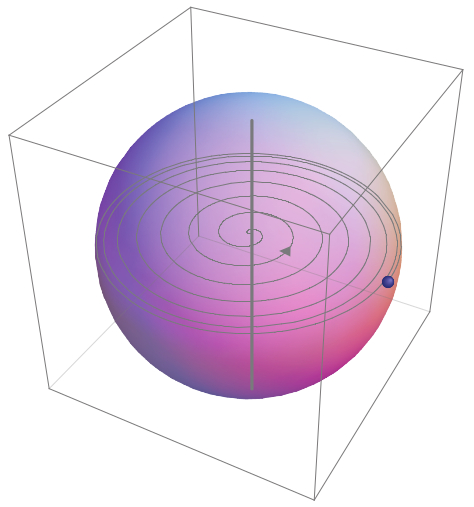
\includegraphics[scale=0.25]{graphics/blochsphere_independance.jpg}\,\cite{Tegmark_15_long}
					\end{column}
				\end{columns}}{}
				
		\alt<3>{\begin{beamerboxesrounded}{Unabhängigkeits-Paradoxon}
				Zerlegt man das Universum in maximal unabhängige Objekte,
				kommt jegliche Veränderung zum erliegen.
			\end{beamerboxesrounded}}{}
\end{frame}